
\section{Experiments}
\label{secn:experiments}

We start this investigation by explaining very shortly the project structure for this exercise. Unlike analysis where notebooks were used, Python files were used to create the models, tune them and carry out experiments. 


\begin{itemize}
	\item A \textbf{utils} area contains all the scripts necessary to download the dataset, split it in train and test datasets, define the feature engineering module and create the preprocessing pipeline. As most of these scripts manipulate the dataset, their result is ultimately saved in a \textbf{data} folder.
	
	\item A \textbf{models} area contains the definition of the k-nearest neighbour, logistic regressor and neural network. In all three model definitions, an initial step is to try and access a 'best parameters' file that contains the result of an optimization step that is described later on in this list. The model is combined with the preprocessor  to create the particular model pipeline.
	
	\item An \textbf{experiments} area contains all the experiments that are carried out as part of this exercise. It contains three types of modules:
	
	\begin{enumerate}
		\item A script is designed to evaluate the performance of a machine learning pipeline on test data. It computes and reports key metrics, including accuracy, ROC AUC, F1-scores for both  classes, precision, overall accuracy, and weighted average F1. The evaluation includes generating and saving a classification report, a confusion matrix image, and an ROC curve graph. Results are saved in the \textbf{results} folder.
		
		\item \textbf{Experiment} scripts for each of the three machine learning methods that is used for training, evaluating, and saving a model pipeline. It loads the training and test datasets, fits the specified model pipeline on the training data, evaluates its performance on the test data using the functions explain previously, and saves the trained pipeline to a file.
		
		\item \textbf{Optimization} scripts that tunes the machine learning model pipelines using grid search with cross-validation. After completing the grid search, each script saves the best parameters and corresponding cross-validation accuracy. It also exports the full results of the grid search as a CSV file. This process is carried out to select the optimal model hyperparameters.
	\end{enumerate}
\end{itemize}



%pipeline
%--------


\subsection{Preparing data for machine learning}

Building on the insights derived from the previous section, the next step involved the creation of the pipeline to transform the raw dataset into a format optimized for machine learning models.

\begin{figure}[H]
	\centering
	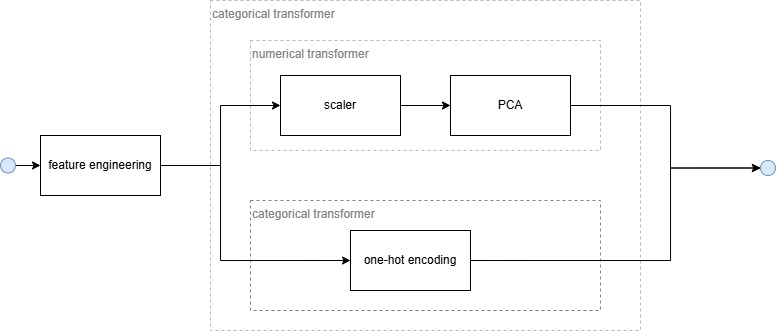
\includegraphics[width=0.7\linewidth]{img/pipeline}
	\caption{The data transformation pipeline for this project.}
	\label{fig:pipeline}
\end{figure}

The pipeline created for this application is shown in Figure \ref{fig:pipeline}. It is based on the \texttt{Pipeline} functionality provided by the Scikit-learn library, integrating feature engineering and transformations for both numerical and categorical data. The pipeline consists of the following components:

\begin{itemize}
	\item \textbf{Feature Engineering:}
	The pipeline begins with a feature engineering unit where raw features are processed to derive new attributes and filter out irrelevant ones. This step prepares the dataset for subsequent transformations. Feature engineering is based on the Python’s \texttt{pandas} library. The transformation logic was encapsulated in a reusable function, \texttt{feature\_engineering}, which was wrapped in a \texttt{FunctionTransformer} to integrate it into  the machine learning pipeline. 
	
	The primary objective of the feature engineering step is to:
	\begin{itemize}
		\item Retain only the most relevant features for recidivism prediction.
		\item Derive new features to enhance the dataset’s predictive capacity.
		\item Remove unnecessary or redundant columns to reduce noise and complexity.
	\end{itemize}
	
	Following the analysis phase, a subset of the dataset's features was identified as relevant for training and subsequent analysis. These include demographic attributes (e.g., \texttt{age}, \texttt{race}, \texttt{sex}), prior criminal history (\texttt{priors\_count}), juvenile offense counts (\texttt{juv\_fel\_count}, \texttt{juv\_misd\_count}, \texttt{juv\_other\_count}), and timestamps related to jail custody (\texttt{c\_jail\_in}, \texttt{c\_jail\_out}) and general custody (\texttt{in\_custody}, \texttt{out\_custody}). Features such as names and IDs were excluded to avoid introducing irrelevant or sensitive information into the analysis.
	
	We decided to keep the \texttt{race} feature so that we can use it to analyse the results obtained by the machine learning models, but it will be removed from the features set at a later stage.
	
	Two new features were created to capture time-based patterns:
	\begin{itemize}
		\item \textbf{\texttt{days\_in\_jail}}: Calculated as the absolute difference in days between the \texttt{c\_jail\_in} and \texttt{c\_jail\_out} timestamps. This feature provides insight into the duration of incarceration for a given charge.
		\item \textbf{\texttt{days\_in\_custody}}: Calculated as the absolute difference in days between the \texttt{in\_custody} and \texttt{out\_custody} timestamps. This feature reflects the total time an individual spent in custody.
	\end{itemize}
	
	These features offer information about the extent of an individual’s interaction with the criminal justice system, which may correlate with recidivism likelihood. As the originating features  had frequent nulls, zeros were imputed where the calculation did not result into a number.
	
	The final processed dataset contains the following columns:
	\begin{itemize}
		\item \textbf{Demographic Features}: \texttt{sex}, \texttt{age}, \texttt{race}.
		\item \textbf{Juvenile Offense Counts}: \texttt{juv\_fel\_count}, \texttt{juv\_misd\_count}, \texttt{juv\_other\_count}.
		\item \textbf{Criminal History}: \texttt{priors\_count}.
		\item \textbf{Derived Features}: \texttt{days\_in\_jail}, \texttt{days\_in\_custody}.
	\end{itemize}
	
	This feature engineering process resulted in a clean and concise dataset, ready for use in machine learning pipelines. By deriving meaningful features and eliminating irrelevant data, the preprocessing step set a strong foundation for building predictive models.
	
	
	\item \textbf{Numerical transformer:}
	\begin{itemize}
		\item \textbf{Scaler:} Numerical features are standardized or normalized to ensure they are on a similar scale. This step is critical for distance-based algorithms and gradient-based optimization.
		\item \textbf{PCA (Principal Component Analysis):} After scaling, dimensionality reduction is applied to numerical features to eliminate redundancy and reduce the complexity of the data. PCA retains the most important components that explain the majority of variance in the data.
	\end{itemize}
	
	\item \textbf{Categorical Transformer:}
	\begin{itemize}
		\item \textbf{One-Hot Encoding:} Categorical variables are transformed into numerical format using one-hot encoding. This technique creates binary columns for each category, ensuring compatibility with machine learning models.
	\end{itemize}
	
	\item \textbf{Integration of Transformations:}
	The outputs from the \textit{numerical transformer} and \textit{categorical transformer} are combined into a unified dataset using the Scikit-learn pipeline framework. This ensures that the transformations are consistently applied to both training and testing datasets, improving reproducibility and minimizing data leakage.
\end{itemize}

This pipeline structure allows for the independent processing of numerical and categorical features, enabling specialized transformations for each type of data. The modular design, powered by Scikit-learn’s \texttt{Pipeline} and \texttt{ColumnTransformer}, ensures flexibility and reusability, making it adaptable to various datasets and machine learning workflows. By incorporating scaling, PCA, and encoding, the pipeline ensures the dataset is well-prepared, reducing potential biases or inefficiencies during model training.

This approach represents an effective preprocessing strategy for heterogeneous datasets and highlights the importance of tailored transformations for achieving robust model performance.



\bigskip
\subsubsection{Logistic regression experiments}

Logistic regression results demonstrate that the model achieved a test accuracy of approximately 69.5\%, and a ROC AUC of 0.74 as can be seen in Figure \ref{fig:logisticregressionroc}, outperforming the baseline COMPAS results in several key areas. The logistic regression model demonstrated better overall accuracy compared to COMPAS and a higher ROC AUC, and therefore improved discriminatory power in separating the two classes. Furthermore, the F1-score for the minority class was significantly higher, reflecting a better balance between precision and recall, particularly for the harder-to-predict positive class.

\begin{figure}[H]
	\centering
	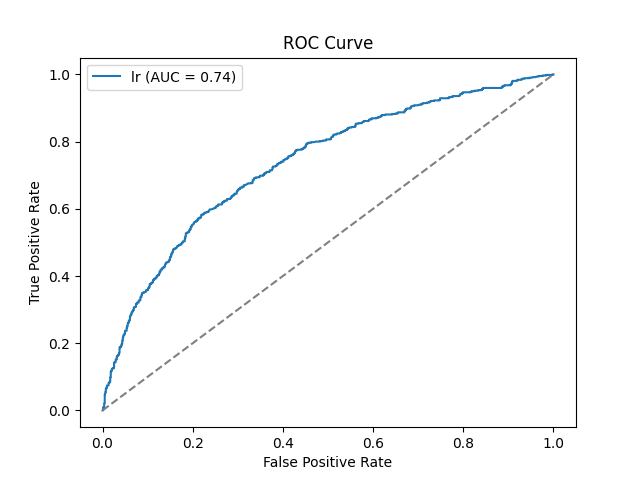
\includegraphics[width=0.7\linewidth]{img/logistic_regression_roc}
	\caption{Receiver operator characteristic plot for logistic regression model}
	\label{fig:logisticregressionroc}
\end{figure}


Examining the confusion matrix show in Figure \ref{fig:logisticregressioncm} we can see that the logistic regression model's improvements. The tuned model identified fewer false positives and false negatives relative to the COMPAS predictions, suggesting that logistic regression was more effective at minimizing classification errors across both classes. The tuned model demonstrated better precision and recall for class 1 (minority), whereas COMPAS appears to struggle more with recall, as it has a larger number of false negatives. This is a significant improvement as false negatives correspond to the people that has a high decile score but did not have further encounters with the legal system.

\begin{figure}[H]
	\centering
	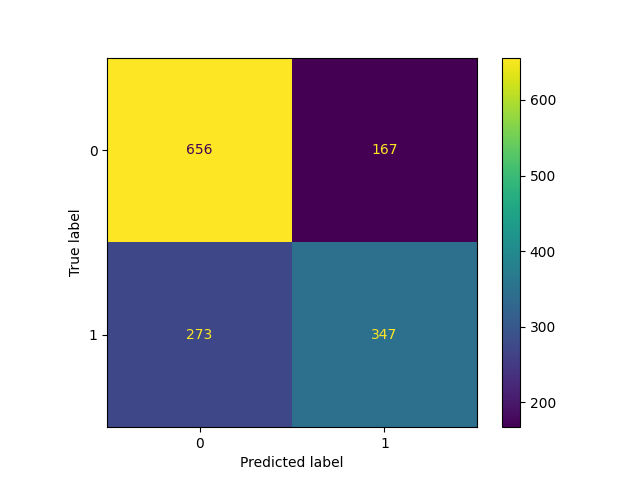
\includegraphics[width=0.7\linewidth]{img/logistic_regression_cm}
	\caption{Confusion matrix for logistic regression model}
	\label{fig:logisticregressioncm}
\end{figure}


The \texttt{class\_weight='balanced'} parameter in Scikit-learn's \texttt{LogisticRegression} adjusts the weights of the classes to be inversely proportional to their frequencies in the training data, hence attempting to address class imbalance. By assigning higher importance to the minority class 1, this parameter ensures that the model does not disproportionately favour the majority class 0. As a result, the recall for class 1 improved to 0.67 compared to previous configurations, indicating that the model is better at correctly identifying instances of the minority class. However, this improvement came at a slight cost to precision for both classes, as the model now predicts class 1 more frequently, leading to a lower overall accuracy (67.71\%). 

With the balanced weights, the model's improved recall for the minority class, that is the individuals who will reoffend, may lead to better proactive interventions. However, the trade-off is an increase in false positives, which could mean incorrectly labelling individuals as high risk. This could unfairly subject some individuals to harsher penalties

This result is a clear indicator of the ethical and societal implications of optimizing machine learning models, especially for imbalanced datasets like this one.



\bigskip
\subsubsection{K-nearest neighbour experiments}

The KNN model outperformed both logistic regression and COMPAS, achieving a test accuracy of 73.46\% and a ROC AUC of 0.80. With an F1-score of 0.66 for the minority class, KNN demonstrated a better balance between precision and recall, improving classification fairness. Its strong discrimination ability (AUC = 0.80) suggests that KNN is more effective in distinguishing between recidivists and non-recidivists.

\begin{figure}[H]
	\centering
	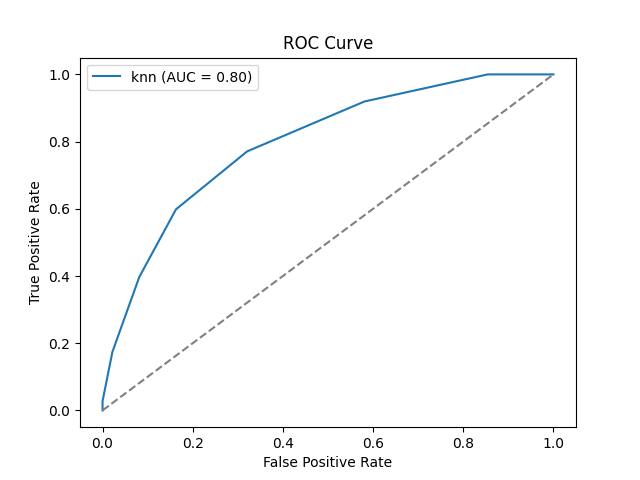
\includegraphics[width=0.7\linewidth]{img/knn_roc}
	\caption{Receiver operator characteristic plot for k-nearest neighbour model}
	\label{fig:knnroc}
\end{figure}

Compared to logistic regression, the confusion matrix for kNN, shown in Figure \ref{fig:knncm} shows fewer false positives and a higher number of true positives. This suggests that kNN is better at minimizing classification errors for the majority class while still improving recall for the minority class. Compared to COMPAS, kNN drastically reduces false negatives and false positives, making it a significantly more balanced and fair model for this classification task.

In practical terms, the improved performance of kNN translates to more accurate predictions, particularly for identifying individuals at higher risk. This could lead to better decision-making, reducing the likelihood of unfairly labeling low-risk individuals as high risk while improving the identification of true high-risk cases. 	


\begin{figure}[H]
	\centering
	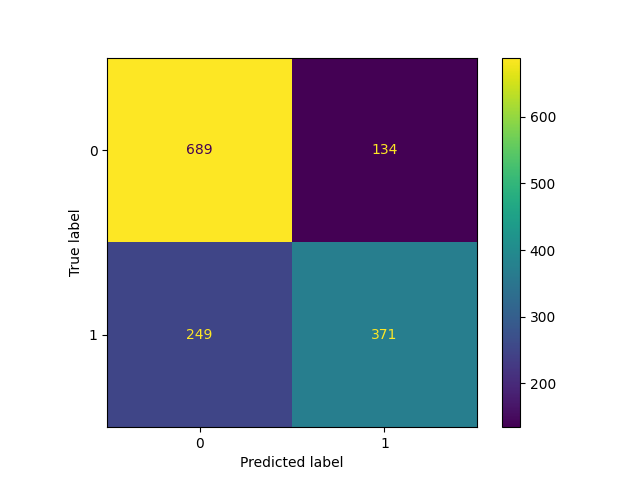
\includegraphics[width=0.7\linewidth]{img/knn_cm}
	\caption{Confusion matrix for k-nearest neighbour model}
	\label{fig:knncm}
\end{figure}



The KNN model with \texttt{weights='distance'} achieved an AUC of 0.9991, suggesting extreme overfitting. While precision and recall were near-perfect, the model likely memorized the training data rather than learning generalizable patterns. This raises fairness concerns, as overfitting could amplify dataset biases. Future work should explore regularization techniques to improve model robustness.

\begin{figure}[H]
	\centering
	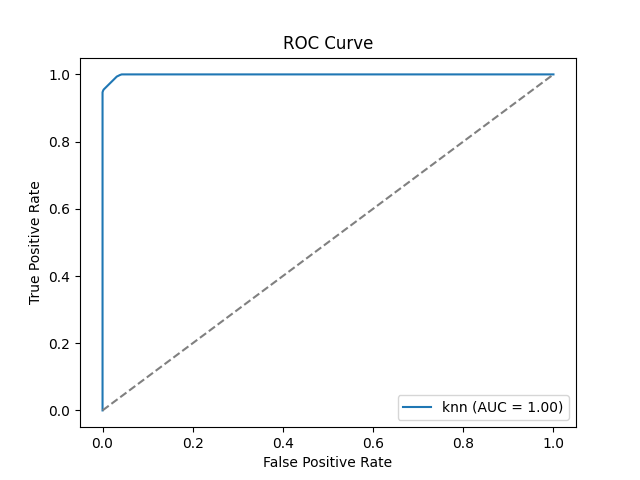
\includegraphics[width=0.7\linewidth]{img/knn_roc_distance}
	\caption{Receiver operator characteristic plot for k-nearest neighbour model with weights parameter set to distance. This is probably the result of overfitting.}
	\label{fig:knnrocdistance}
\end{figure}


\begin{figure}[H]
	\centering
	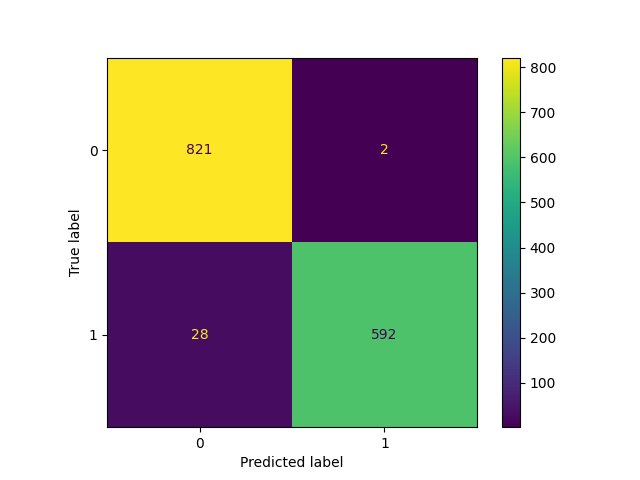
\includegraphics[width=0.7\linewidth]{img/knn_cm_distance}
	\caption{Confusion matrix for k-nearest neighbour model with weights parameter set to distance. This is probably the result of overfitting.}
	\label{fig:knncmdistance}
\end{figure}

\bigskip
\subsubsection{Neural network experiments}

The neural network implemented in exercise consists of an input layer, followed by two fully connected hidden layers. The first hidden layer contains 128 neurons, and the second contains 64 neurons, each followed by batch normalization and a ReLU activation function. The output layer consists of 2 neurons with a softmax activation function. The model is trained using the cross-entropy loss function, optimized with the Adam optimizer, and employs a mini-batch training strategy with a default batch size of 32 and 20 epochs.

The neural network achieved a test accuracy of 70\% and an AUC of 0.75, demonstrating moderate classification performance. While recall for the minority class improved (0.69), the model still exhibited a higher misclassification rate compared to KNN. The confusion matrix revealed 242 false positives and 191 false negatives, indicating room for further optimization.


\begin{figure}[H]
	\centering
	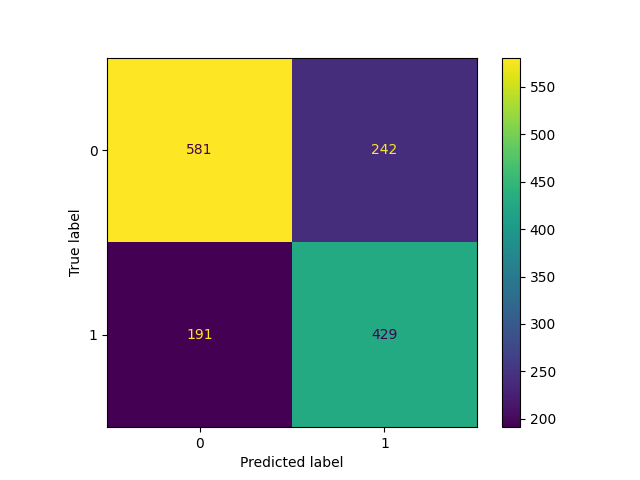
\includegraphics[width=0.7\linewidth]{img/nn_cm}
	\caption{Confusion matrix for neural network model.}
	\label{fig:nncm}
\end{figure}

\begin{figure}[H]
	\centering
	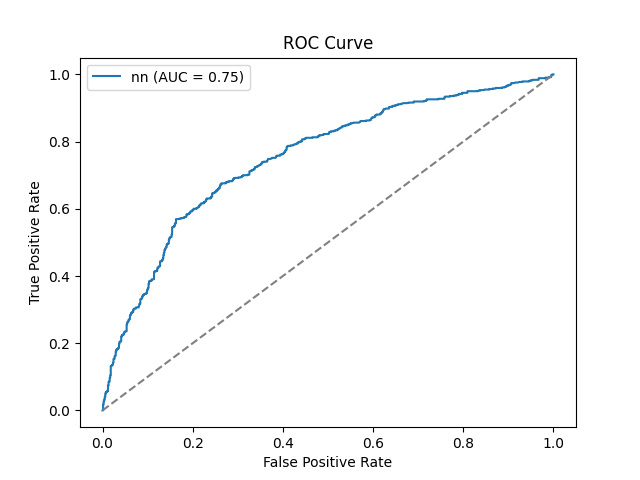
\includegraphics[width=0.7\linewidth]{img/nn_roc}
	\caption{Receiver operator characteristic plot for neural network model.}
	\label{fig:nnroc}
\end{figure}


Changing the loss function to mean squared error caused some differences in how the network performs. While the overall accuracy stayed the same, the model became better at identifying instances of the minority class but less precise when predicting the majority class. This happens because MSE treats errors more evenly, which helps the model focus on reducing overall mistakes rather than just making the most confident predictions.

By using MSE, the model seems to make fairer predictions across both classes, improving recall for the minority class. However, this comes with a trade-off; we may not be as confident in its predictions. Choosing MSE or another loss function depends on what matters most for the task—whether it's catching as many minority cases as possible or making highly confident predictions.

\subsubsection{Final comments on experiments}

Table \ref{tab:metrics} summarizes the performance metrics across the different techniques.


\begin{table}[H]
	\centering
	\begin{tabular}{|l|c|c|c|c|}
		\hline
		\textbf{Technique} & 
		\makecell{F1-Score \\Class 0\\Class 1} & 
		\makecell{Precision \\ (Class 1)} & 
		\makecell{Overall\\Accuracy} & 
		\makecell{Weighted\\Avg\\F1-Score} \\ \hline
		lr & \makecell { 0.75 \\ 0.61 } & 0.68 & 0.70 & 0.68 \\ \hline
		lr balanced & \makecell { 0.71 \\ 0.64 } & 0.61 & 0.68 & 0.67 \\ \hline
		knn & \makecell { 0.78 \\ 0.66 } & 0.73 & 0.73 & 0.72 \\ \hline
		knn distance & \makecell { 0.98 \\ 0.98 } & 1.00 & 0.98 & 0.98 \\ \hline
		nn & \makecell { 0.76 \\ 0.62 } & 0.66 & 0.70 & 0.69 \\ \hline
		nn mse& \makecell { 0.72 \\ 0.68 } & 0.63 & 0.70 & 0.70 \\ \hline
	\end{tabular}
	\caption{Performance Metrics for Classification Techniques}
	\label{tab:metrics}
\end{table}


The k-Nearest Neighbors (\texttt{knn}) model performed better than logistic regression in both overall accuracy and weighted F1-score, with a significant improvement in capturing minority class instances. The use of distance-based weights (\texttt{knn distance}) led to exceptional performance, with near-perfect metrics across all evaluation categories. However, this result indicates overfitting and should be carefully validated on more data.

The neural network (\texttt{nn}) achieved comparable performance to logistic regression, with a slight improvement in recall for the minority class. Changing the loss function to mean squared error (\texttt{nn mse}) resulted in a better balance between precision and recall for both classes, leading to a slight improvement in the weighted F1-score compared to the cross-entropy loss variant. This suggests that MSE as a loss function can encourage fairer predictions across classes in certain scenarios.

Overall, \texttt{knn} outperformed \texttt{lr} and \texttt{nn} models in most metrics, with \texttt{nn mse} demonstrating improved balance compared to \texttt{nn}. However, the extremely high metrics of \texttt{knn distance} should be interpreted with caution, as they may not generalize well to unseen data. The choice of model and loss function should depend on the specific application and the importance of precision, recall, and generalization.
